\documentclass{article} 
\usepackage{nips15submit_e}
\usepackage{hyperref}
\usepackage{amsmath}
\usepackage{url}
\usepackage{graphicx}
\usepackage{tabularx}
\usepackage{placeins}
%\documentstyle[nips14submit_09,times,art10]{article} % For LaTeX 2.09
\usepackage{filecontents}



%%%%%%%%%%%%%%%%%%%Bibliography%%%%%%%%%%%%%%%%%%%%%%%%%
\begin{filecontents}{Sta561_FinalProject_DreamTeam.bib}
@article{paper1,
author={Yehezkel Dar and Nura Resh},
title="{Classroom Intellectual Composition and Academic Achievement}",
journal={American Educational Research Journal},
volume={23},
number={3},
pages={357-374},
year={1986}
}

@article{paper2,
author = {Amita Chudgar and Thomas F. Luschei and Yisu Zhou},
title = "{Science and Mathematics Achievement and the Importance of Classroom Composition: Multicountry Analysis Using TIMSS 2007}",
journal = {American Journal of Education},
year = {2013},
volume = {119},
number = {2},
pages = {295-316},
month = {Feb}
}

@article{paper3,
author = {Robert Dreeben and Rebecca Barr},
title = "{Classroom Composition and the Design of Instruction}",
journal = {Sociology of Education},
year = {1988},
volume = {61},
number = {3},
pages = {129-142},
month = {Jul}
}

@Manual{step, 
    title = {MASS: Support Functions and Datasets for Venables and Ripley's MASS}, 
    author = {Brian Ripley and Bill Venables and Douglas M. Bates and Kurt Hornik (partial port ca 1998) and Albrecht Gebhardt (partial port ca 1998) and David Firth}, 
    year = {2015}, 
    note = "R package version 7.3-45, \url{http://CRAN.R-project.org/package=MASS}"
} 


@Manual{mice, 
    title = {mice: Multivariate Imputation by Chained Equations}, 
    author = {Stef van Buuren and Karin Groothuis-Oudshoorn and Alexander Robitzsch and Gerko Vink and Lisa Doove and Shahab Jolani}, 
    year = {2015}, 
    note = "R package version 2.25, \url{http://CRAN.R-project.org/package=mice}"
} 


@Article{lasso,
author = {Robert Tibshirani},
title = "{Regression Shrinkage and Selection via Lasso}",
journal = {Journal of the Statistical Society. Series B(Methodological)},
year = {1996},
volume = {58},
number = {1},
pages = {267-288}
}

@article{ridge,
author = {Donald W. Marquardt and Ronald D. Snee},
title = "{Ridge Regression in Practice}",
journal = {The American Statistician},
year = {1975},
volume = {29},
number = {1},
pages = {3-20},
note = "\url{http://www.jstor.org/stable/2683673}"
}

@article{elasticnet,
author = {Hui Zou and Trevor Hastie},
title = "{Regularization and variable selection via the elastic net}",
journal = {Journal of the Royal Statistical Society, Series B},
year = {2005},
volume = {67},
pages = {301-320},
note = "\url{https://web.stanford.edu/~hastie/Papers/elasticnet.pdf}"
}

@Article{paper4,
author = {Jennifer L. DePaoli and Joanna Hornig Fox and Erin S. Ingram and Mary Maushard and John M. Bridgeland and Robert Balfanz},
title = "{Building a Grad Nation(Progress and Challenge in Ending the High School Dropout Epidemic)}",
note = "{Instituitions: Civic Enterprisesa and Everyone Graduates Center at the School of Education at Johns Hopkins University}",
month = {May},
year = {2015}
}

@misc{wiki,
  author = {Wikipedia},
  title = "Stepwise regression --- {W}ikipedia{,} The Free Encyclopedia",
  year = 2015,
  howpublished = {\url{https://en.wikipedia.org/wiki/Stepwise_regression}},
  note = "[Online; accessed 14-November-2015]"
}

@article{aic,
author = {Hirotugu Akaike},
title = "{A New Look at the Statistical Model Identification}",
journal = {IEEE TRANSACTIONS ON AUTOMATIC CONTROL},
year = {1974},
volume = {19},
number = {6},
pages = {716-723},
month = {Dec}
}
\end{filecontents}
%%%%%%%%%%%%%%%%%%%%End Bibliography%%%%%%%%%%%%%%%%%%%%%%%



\title{The Effect of Racial Diversity on Graduation Rates in U.S. School Districts}

\author{
Sanjay Hariharan \\
Department of Statistics\\
Duke University\\
\texttt{sanjay.hariharan@duke.edu} \\
}

% The \author macro works with any number of authors. There are two commands
% used to separate the names and addresses of multiple authors: \And and \AND.
%
% Using \And between authors leaves it to \LaTeX{} to determine where to break
% the lines. Using \AND forces a linebreak at that point. So, if \LaTeX{}
% puts 3 of 4 authors names on the first line, and the last on the second
% line, try using \AND instead of \And before the third author name.

\newcommand{\fix}{\marginpar{FIX}}
\newcommand{\new}{\marginpar{NEW}}

\nipsfinalcopy 

\begin{document}

\maketitle


\begin{abstract}
In this paper we assess whether a statistic designed to measure the holistic level of racial diversity in a school district has a statistically significant impact on the graduation rate in the school district.  The analysis is performed using data from the Data for Diplomas project, which is an amalgamation of data from various sources, including the 2010 US census and the American Community Survey.  
\end{abstract}


\section{Introduction}\label{background}

In the education literature there are various theories about the effect of classroom composition \cite{paper2} on education outcomes, such as graduation rate or test scores. One paradigm for measuring classroom composition is racial diversity.  We are interested in exploring the relationship between racial diversity and education outcomes\cite{paper1}.

In this paper, we propose a measure of racial diversity and attempt to explore the relationship between this statistic and graduation rates across school districts in the United States. We expect a small but significant relationship between these two factors. In our analysis, we explore the relationship between these factors, devoting special attention to controlling for potentially confounding economic variables. 


 \subsection{Data Cleaning}\label{dataset}
This data set was very challenging to work with and exhibited many problems common to large data sets.  The data set was created by merging together information on high schools by school districts along with census information. Census information is not classified by school districts, so the two dataset were matched by degree of geographic overlap.  The most challenging problem with the data set was missing data.  We used the VIM packages in R to assess the missing data.  We found that numerous feature columns had missing data in different proportions.  We decided to drop observations with missing values for graduation rates (the response variable in our regression). Feature columns with small amount of missing data ($<$ 2\%) were assumed to be 0. 

Unfortunately, the columns with the largest quantity of missing data were the features that contained information on the racial composition of the students in the school district.  This posed a serious problem, as we used this information to compute the diversity statistic. Since the diversity statistic is the central predictor in our model, omitting all observations with missing data is simply not possible; this would result in a loss of approximately a two-thirds of our data.  Since we had information on the racial composition of the district on the population level from the census data, we decide to impute the missing data on racial composition of the students using multivariate imputation by chained equations (MICE) implemented by the \texttt{mice} package in R \cite{mice}.  We created 50 different datasets with imputed values. We were glad to find that the diversity statistics was fairly stable under all the datasets (see Figure \ref{4hists}).  This approach relies on the assumption that the racial composition of the school district is similar to the racial composition of the community at large, which may not be entirely accurate, given the structure of the data set.

\section{Understanding Diversity}

We attempt to construct a general measure of diversity that will be high for racially diverse communities and low for racially homogeneous communities.  By doing this, we hope to construct results that can be seen without reference to specific ethnic groups.  We define the diversity statistic $D_j$ for community $j$ to be
\begin{align*}
 D_j = \prod_{i \in I}(1-x_{i,j}),
\end{align*}

where $I$ is an indexing set for ethnic groups and $x_{i,j}$ is the proportion of ethnic group $i$ in community $j$.  We want to determine whether $D_j$ has a statistically significant impact on graduation rates once other factors are accounted for.  

The use of such a statistic may be desirable due to the correlation between ethnicity and wealth.  Since wealth is highly correlated with positive academic outcomes, there is a concern that the ethnic composition of a community maybe serving as  a proxy for wealth in our analysis.  We want to establish whether the level of diversity (measured using $D_j$) is significant after wealth and other demographic information has been taken into account. Median income and poverty level are among the first covariates we control for in our analysis.

\section{Inference}

In order to assess the relationship between racial diversity and graduation rates we ran regression models of varying complexity. Due to the high level of missing data, we created 50 different imputed data sets (see Section \ref{dataset}).  The regressions are performed across all data sets to account for variability.  Table \ref{regresults} presents relevant summary statistics for the estimated coefficient for Diversity. These values are averaged over all 50 imputed data sets.

\begin{table}[ht]
\caption{Regression summary}
\label{regresults}
\centering
\begin{tabular}{rrrrrr}
  \hline
Model & Mean & Variance & Std. Error & t value & p value \\ 
  \hline
Linear 1 & -59.97 & 0.65 & 1.39 & -43.28 & 0.00 \\ 
  Linear 2 & -53.36 & 0.81 & 1.36 & -39.29 & 0.00 \\ 
  Linear 3 & -69.56 & 2.92 & 2.48 & -28.04 & 0.00 \\ 
   Linear 4 & -59.33 & 0.57 & 1.38 & -43.09 & 0.00 \\ 
  Linear 5 & -75.43 & 1.19 & 2.14 & -35.21 & 0.00 \\ 
  Linear 6 & -85.41 & 3.46 & 3.01 & -28.34 & 0.00 \\ 
  Lasso 1 & -45.04 & 2.18 & 1.47 & -30.57 & 0.00 \\
  Lasso 2 & -62.23 & 499.20 & 20.37 & -3.12 & 0.03 \\
  Lasso 3 & 62.38 & 530.68 & 22.11 & 2.87 & 0.06 \\
   \hline
\end{tabular}
\end{table}
\begin{table}
\caption{Description of Regression Models}
\label{modeldesc}
\centering
\begin{tabularx}{\textwidth}{l X}
\hline
Model & Covariates \\
\hline
Linear 1 & Regression with diversity as the only covariate \\
Linear 2 & Regression with diversity and median income in the district \\
Linear 3 & Regression with diversity, median income in district, and their interaction \\
Linear 4 & Regression with diversity and the number of people classified as being below the poverty level \\
Linear 5 & Regression with diversity, poverty level, and their interaction \\
Linear 6 & Regression with diversity, poverty, income, and their interactions with diversity \\
\hline
Lasso 1 & Unpenalized regression on variables selected by lasso with the 1 squared error $\lambda$ \\
Lasso 2 & Unpenalized regression on variables selected by lasso (1se) with interaction terms \\
Lasso 3 & Unpenalized regression on variables selected by lasso (1 se) with interaction between all variables and squared terms for each variable \\
\hline
\end{tabularx}
\end{table}

In the linear models 1-6, we attempt to control for economic factors that correlated with diversity. We note however, that we only have information of economic factors at the district level. It maybe preferable to include information for racial groups within the district to entirely control for economic factors. However such information is not available in our data set. 

In all models, diversity is found to be significant, as evidenced by the small p-values on the coefficient estimate. For the relatively simple models, Linear models 1-6 and Lasso 1, the estimate is consistently negative with a low variance, which suggests stability. In Lasso model 3, after adding in squared predictors, we find an interesting result of a positive coefficient estimate. However we also find large variances in our estimates for Lasso 2 and Lasso 3 models. These results suggest instability in the estimates from these models, possibly due to instability in lasso selection methods or increased collinearity from the added interaction and squared terms. We note that $t$ values tend to decrease as model complexity increases.

Nevertheless, the $t$ statistics and $p$-values remain highly significant even when other explanatory variables are included in the model.  This is reasonable evidence that diversity at the district level as we have measured it seems to have a negative relationship with graduation rates.  The quality of inference could perhaps be improved by using a more robust model, such a mixture model.

\subsection{Predictions}

We experimented with a variety of different models to assess the best predictive ability with our data. The total rate of graduation within each school district is our response, with all the other covariates in our dataset fixed. This section provides an overview of the different models we used and our rational behind them.

The first method of model selection we used was lasso.  Given that we have over 350 covariates, the possibility of linear dependence and overfitting is quite high when performing full linear regression. The Lasso of Tibshirani (1996)\cite{lasso} provides a method of variable selection, penalizing covariates and pushing their estimated coefficients to zero. We chose the penalization term $\lambda$ through Cross-Validation, picking the value that minimizes out of sample deviance.

To provide an alternative to our Lasso model, we chose to model the response using Ridge Regression \cite{ridge}, which minimizes the covariate estimated coefficients, but does not zero any out. Like above, we chose the penalization term that minimizes the out of sample deviance.

Since the Lasso Model pushes many coefficient estimates to zero, and the Ridge model keeps all the estimates, we want to compare them against a model that is not so extreme, and rather weighs them equally. The Elastic Net Model does just this, weighing the Ridge and Lasso Regression Penalizations by a value $\alpha$, and choosing the penalization term that minimizes the out of sample deviance \cite{elasticnet}. For our purposes, we chose an equal weight, ie: $\alpha$ = 0.5.

As an substitute for penalized regression, we chose a combination of Forward and Backward Stepwise Selection, called Bidirectional Elimination\cite{step}, and used AIC\cite{aic} as the selection criterion. This method iteratively adds in covariates that best improve the model fit. As covariates are added, the algorithm also removes previous variables that become insignificant compared to the new additions \cite{wiki}.

\subsection{Result}

\begin{figure}[h]
\begin{center}
 \includegraphics[width = .5\textwidth]{graphics/Prediction_BoxPlot.pdf}
\end{center}
\caption{Comparison of Mean Squared Errors \label{boxplot}}
\end{figure}

Data Cleaning with the Mice Package in R resulted in 50 different imputed datasets. Through Cross-Validation, we implemented the four models above on each resulting dataset and computed the Mean Square Error of the model on the known response values. A box plot of the results is presented in Figure \ref{boxplot}.  The mean and variance of the shrinkage parameter across the 50 data sets are presented in Table \ref{lambda}

We can clearly see that the bidirectional elimination model fits our data set the best, followed by the lasso model. This result is due to the fact that both these models completely ignore covariates that do not significantly affect the model. 

Given that our data is public domain, we suspect that the bidirectional-elimination or lasso model would accurately predict graduation rates in future years. Furthermore, our model could be improved with a time series analysis of graduation rates along with our covariates over a number of years.

\begin{table}[ht]
\caption{Penalization values}
\label{lambda}
\centering
\begin{tabular}{r|rr|rr}
  \hline
 & $\lambda_{min}$ & Var($\lambda_{min}$) & $\lambda_{1se}$ & Var($\lambda_{1se}$) \\ 
  \hline
Lasso & 0.04595 & 0.00006 & 0.27143 & 0.00505 \\ 
  Ridge & 1.46487 & 0.03459 & 6.77670 & 1.87964 \\ 
  Elastic Net & 0.08589 & 0.00025 & 0.54794 & 0.01765 \\ 
   \hline
\end{tabular}
\end{table}

\section{Conclusion}

 Despite our best efforts to conduct a rigorous and thorough analysis, there are various potential problems.  One area that may be especially problematic is our data cleaning methods.  We began with a very messy data set and had to impute for large amounts of missing data.
 
 The Ecological Inference Problem is relevant to our analysis. The aggregation of data across districts will tend to amplify the effects of the covariates on the response.  That is to say, the effect of diversity is likely stronger on a district level than it is on a school level.  Our data set does not include information on the number of high schools in each district, so we cannot restrict our attention to those districts with only one high school.  An analysis on the school level might give drastically different results. 
 
We may not have sufficiently controlled factors related to diversity. It is possible that important covariates were lacking and our estimate for the effect of diversity suffers from omitted variable bias.  Moreover, the effect of diversity may be regional in a manner that cannot be controlled by state.  In particular, the attitudes towards racial diversity may differ between the Northern and Southern United States due to historical factors.  
 
 We cannot offer an explanation for the mechanism through which diversity affects graduation rates.  We reiterate that our analysis was performed at the district level subject to various limitations.  Nonetheless, we hope that the results in this paper provide an interesting and reasonable motivation for further study.

\section{Appendix}


\section{Data}

We have obtained data from the Data for Diplomas project. This project released a large data set containing Census, ACS Survey, and education specific data across over ten thousand school districts in the United States \cite{paper4}. Information on Idaho, Oklahoma and Kentucky are absent from the data set. There are over 350 features in the dataset. We are primarily interested in data regarding overall graduation rate and racial composition in each school district.

As we only have data at the district level, it is difficult to make claims about the relationship between diversity and graduation rate in a school because school districts can have multiple high schools, which poses a problem for inference. It could be the case that a racially diverse district contains racially homogeneous schools. In our data set such an observation would appear as a single diverse district.  This type of confounding will tend to strengthen the relationship between diversity and graduation rate, making inference difficult. This problem is exacerbated even more by the fact that students are not randomly assigned to schools. Instead, the majority are assigned to a high school based on residence. As ethnic groups commonly live in close-knit communities, there are likely to be high schools dominated by a distinct racial group \cite{paper3}. 

The data set is rather messy and contains many missing values. A discussion of the procedures used to clean the data and impute missing values can be found in the Appendix in Section \ref{dataset}

 \subsection{Mathematical Properties of the Diversity Statistic}
 Let $I$ be an indexing set containing various ethnic groups and let $x_{i,j}$ be the proportion of the population in community $j$ that belongs to ethnic group $i$.  We define the diversity statistic $D_j$ for community $j$ to be 
\begin{align*}
D_j = \prod_{i \in I}(1-x_{i,j}).
\end{align*}
This is subject to the constraints $x_{i,j}>0$ for all $i$ and $j$ and $\sum_{i \in I}x_{i,j}=1$.  We will show that subject to these constraints the maximum value of $D_j$ occurs when $x_{i,j} = 1/|I|$ for all $i$.  
\begin{figure}[t]
\begin{center}
 \includegraphics[width = .75\textwidth]{graphics/diver4hists.pdf}
\end{center}
\caption{histograms of the diversity measure in four (of 50) randomly selected data sets \label{4hists}}
\end{figure}
We will begin with the more general constraint $\sum_{i \in I} x_{i,j} = c$ with $c \leq 1$.  Fix some $j$.  The Lagrangian is
\begin{align*}
 L(\boldsymbol{x}, \lambda) = \prod_{i \in I}(1-x_i) +\lambda \sum_{i \in I}x_i - \lambda c.
 \end{align*}
This results in first order conditions of the form
\begin{align*}
\frac{\partial L}{\partial x_i} = -\prod_{j \in I-\{i\}}(1-x_j) + \lambda.
\end{align*}
First suppose that $x_j = c$ for some $j \in I$.  In this case all $x_i = 0$ for all $i \neq j$ and the value of the objective function is $1 - c$.  Note that if $x_i=x_j=c/2$ the value of the objective function is $(1-c/2)^2 > 1-c$.  Therefore the maximum does not occur when only one $x_i$ is non-zero and we can restrict our attention to situations when $x_i < c$ for all all $i \in I$; in particular $x_i < 1$.  This allows us use the equations derived from the Lagrangian to conclude that $x_i = x_j$ for all $i,j \in I$.  Using the constraint on the sum we immediately find that $x_i = c/|I|$ for all $i \in I$.  

In other words, the value $D_j$ is maximized when all ethnic groups are equally represented in a community.  Conversely, if there is a community $j$ with only one ethnic group, then $D_j =0$, which is the minimum possible value for $D_j$.  Above we used the more general constraint with $c$ to illuminate the following:  if one racial group makes up some proportion of the community, the diversity statistic is maximized when the remaining ethnic groups are equally represented.  These are appealing properties for a measure of diversity.

\begin{figure}[t]
\begin{center}
 \includegraphics[width = .75\textwidth]{graphics/diver2hists.pdf}
\end{center}
\caption{Diversity measure for the same observation in two randomly selected datasets \label{2hists}}
\end{figure}


\subsection{Empirical Stability of the Diversity Statistic}\label{imperstab}
We have proposed a novel measure of diversity and are concerned that the measure may exhibit undesirable behavior.  It would be desirable to have a measure that is stable under small deviations.  We have generated data sets by imputing many values.  The variability in the imputed values will create small variations in the diversity measure, which we can use to examine the stability of the measure.  First we compare the histograms of the diversity measure in four (of 50) randomly selected data sets, which is presented in Figure \ref{4hists}.  Note that the histograms of the observed measures of diversity are similar across data sets.  This suggests that our measure is relatively stable.  We can also verify that the diversity measure for the same observation in two randomly selected data sets is similar, which is presented in Figure \ref{2hists}.  This is done for two pairs of randomly selected data sets.  The histograms are highly concentrated around zero.  This further suggests that the diversity statistic is robust to small changes in the data.   

\subsection{Visualing Diversity}
Figures \ref{diverplot} and \ref{rateplot} show the value of the diversity statistic and graduation rate for school districts in the United States.  The plot of the diversity measure has features that are intuitively appealing.  For example, the Midwest has very low diversity as measured by our statistic.  Many states in this region of the country are composed almost entirely of Caucasians, and the plot reflects this.  Diversity is also higher in certain urban areas, such as Chicago.  Furthermore, southern states, such as California or Arizona, where a large number of hispanics reside, are observed to have high diversity.


\begin{figure}[h]
 \begin{center}
 \vspace{-140pt}
  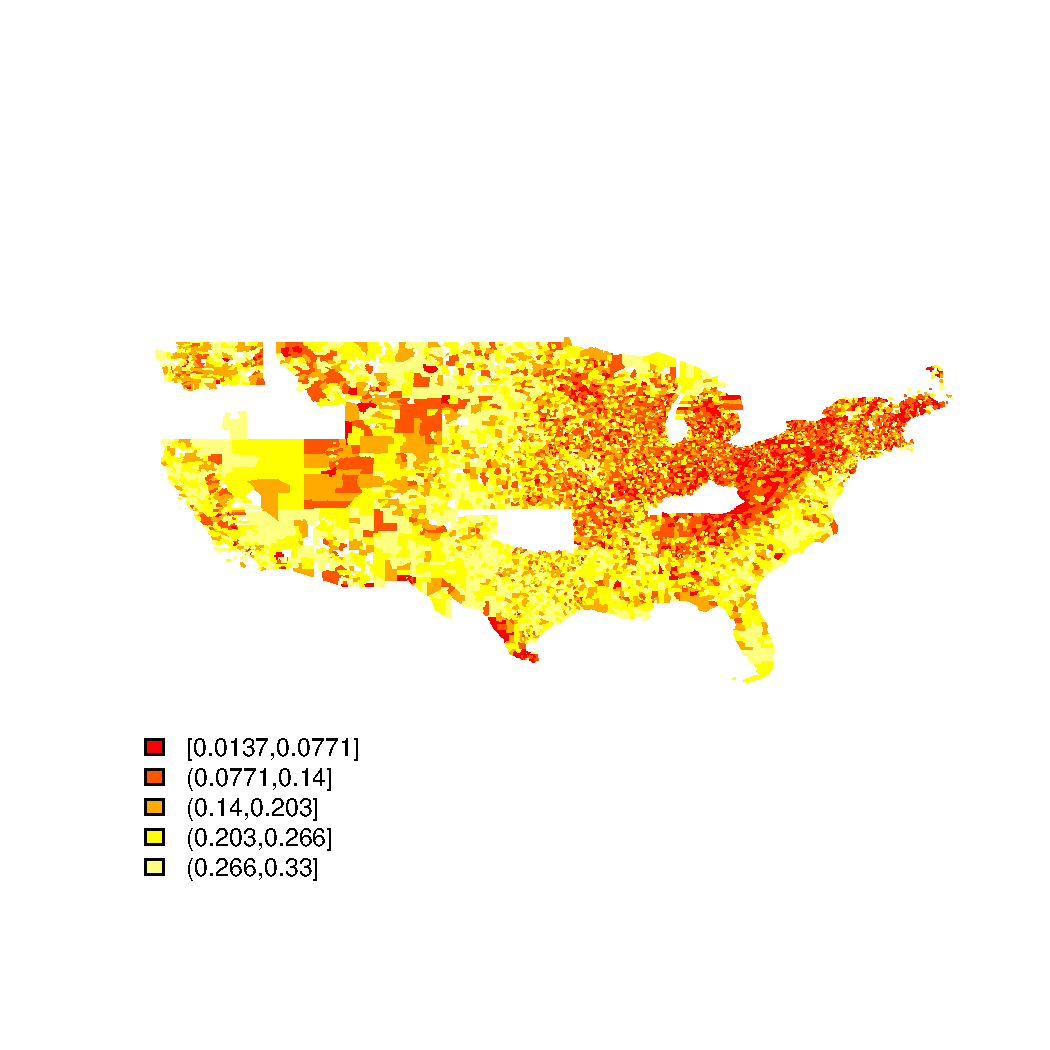
\includegraphics[width = \textwidth]{graphics/USdiverplot.pdf}
 \vspace{-90pt}
 \end{center}
 \caption{Plot of diversity in U.S by school district \label{diverplot}}
\end{figure}


\begin{figure}[h]
 \begin{center}
 \vspace{-140pt}
  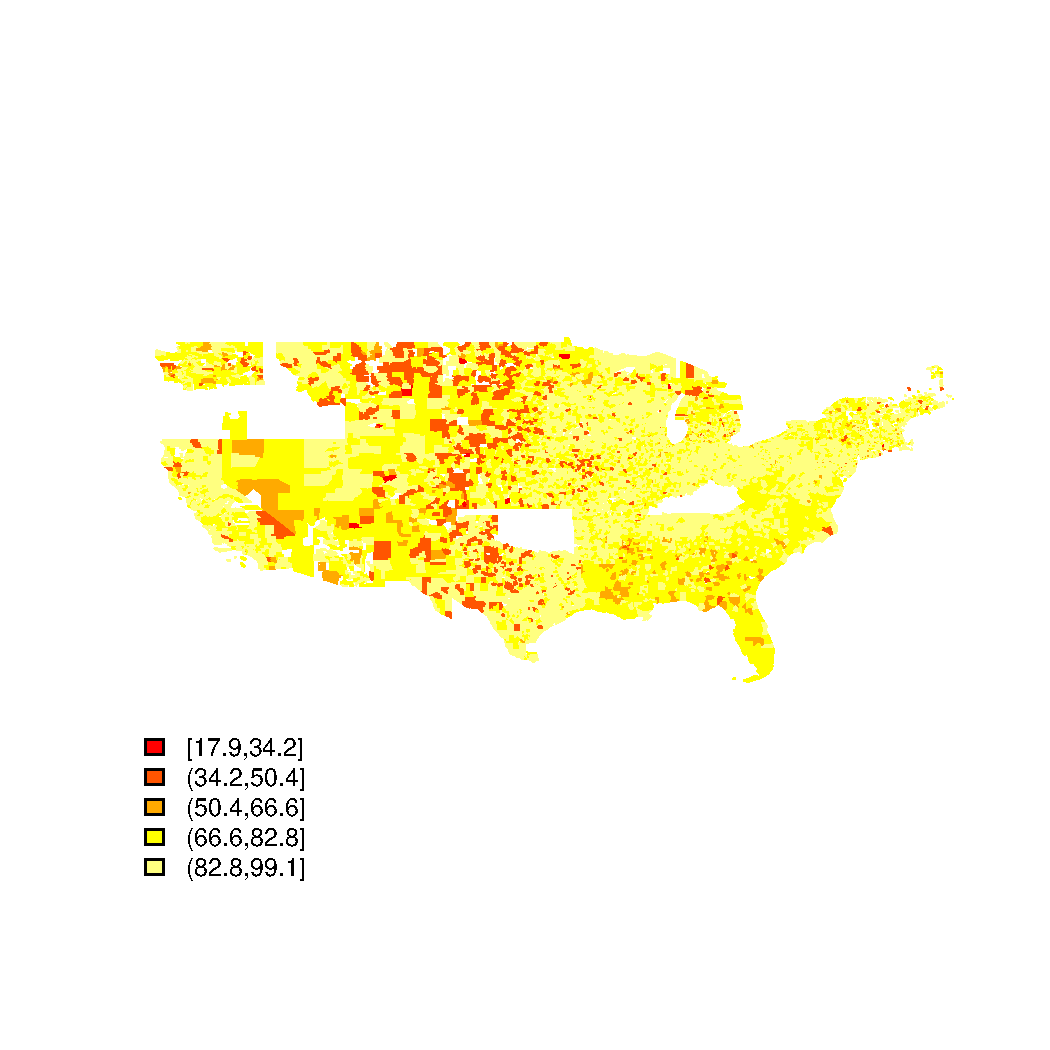
\includegraphics[width = \textwidth]{graphics/USrateplot.pdf}
  \vspace{-90pt}
 \end{center}
 \caption{Plot of graduation rate in U.S by school district \label{rateplot}}
\end{figure}
 


\clearpage % this forces a page break before the bibliography
\bibliographystyle{unsrt}
\bibliography{Sta561_FinalProject_DreamTeam}
\end{document}
